\documentclass[10pt]{article}
\usepackage{caption}
\usepackage{lipsum}
\usepackage{multicol}
\usepackage{amsmath,amssymb,amsthm}
\usepackage{graphicx}
\usepackage[margin=1in]{geometry}
\usepackage{ragged2e}

\begin{document}

\title{\textbf{Hedging Uniswap Liquidity Positions with GMX Perpetuals}}
\author{\textbf{Xtreamly}}
\date{\today}
\maketitle

\begin{abstract}
	This paper explores the use of perpetual futures to hedge Uniswap V4 and V3 concentrated liquidity positions. By integrating short perpetual strategies with Xtreamly’s volatility predictions, liquidity providers can mitigate impermanent loss and potentially profit from price fluctuations. We analyze the effects of volatility forecasts, leverage, funding costs, and liquidation risks on effective risk management. Finally, we apply the hedging strategy to historical LP positions and evaluate its potential to improve the performance.
\end{abstract}
\medskip
\begin{multicols}{2}

\section{Hedging Framework}
\label{sec:hedging}

We propose a hedging mechanism that combines Uniswap V4 \& V3 liquidity provider (LP) positions with GMX perpetual futures to reduce risk and enhance performance. This section outlines the key components of the strategy: the Uniswap LP position, the GMX perpetual futures contract, and Xtreamly’s volatility forecasting component.

\subsection{Uniswap LP Position}
\label{sec:uniswaplp}

\subsubsection{Overview}
Consider a LP position in the Uniswap pool within \textit{concentrated liquidity} (CL) as the liquidity is bounded within a range of lower and upper price. To keep real world intuition, let \textbf{ETH ($token_0$)} represent the volatile asset and \textbf{USDT ($token_1$)} be the stable  asset value for the pools currently considered for hedging.

\subsubsection{LP Collected fees}
Collected fees represent the income of an LP position, serving as a reward for providing liquidity and contributing to the position’s final profitability. As long as the market price $P$ remains within the LP position’s upper and lower bounds, the position accrues fees, which enhance the total return. 

\medskip

However, at a given moment $t$ after opening the LP position, with a realized price $P$, these fees do not affect the position’s value at that specific moment (but add up to PnL).

\subsubsection{LP Impermanent Loss}

Impermanent loss (IL) occurs when the prices of tokens in a liquidity pool diverge from their initial values at the time of liquidity provision, reducing the LP position’s value. For simplicity, we exclude entry fees, gas fees, and collected fees from this analysis, focusing solely on IL.

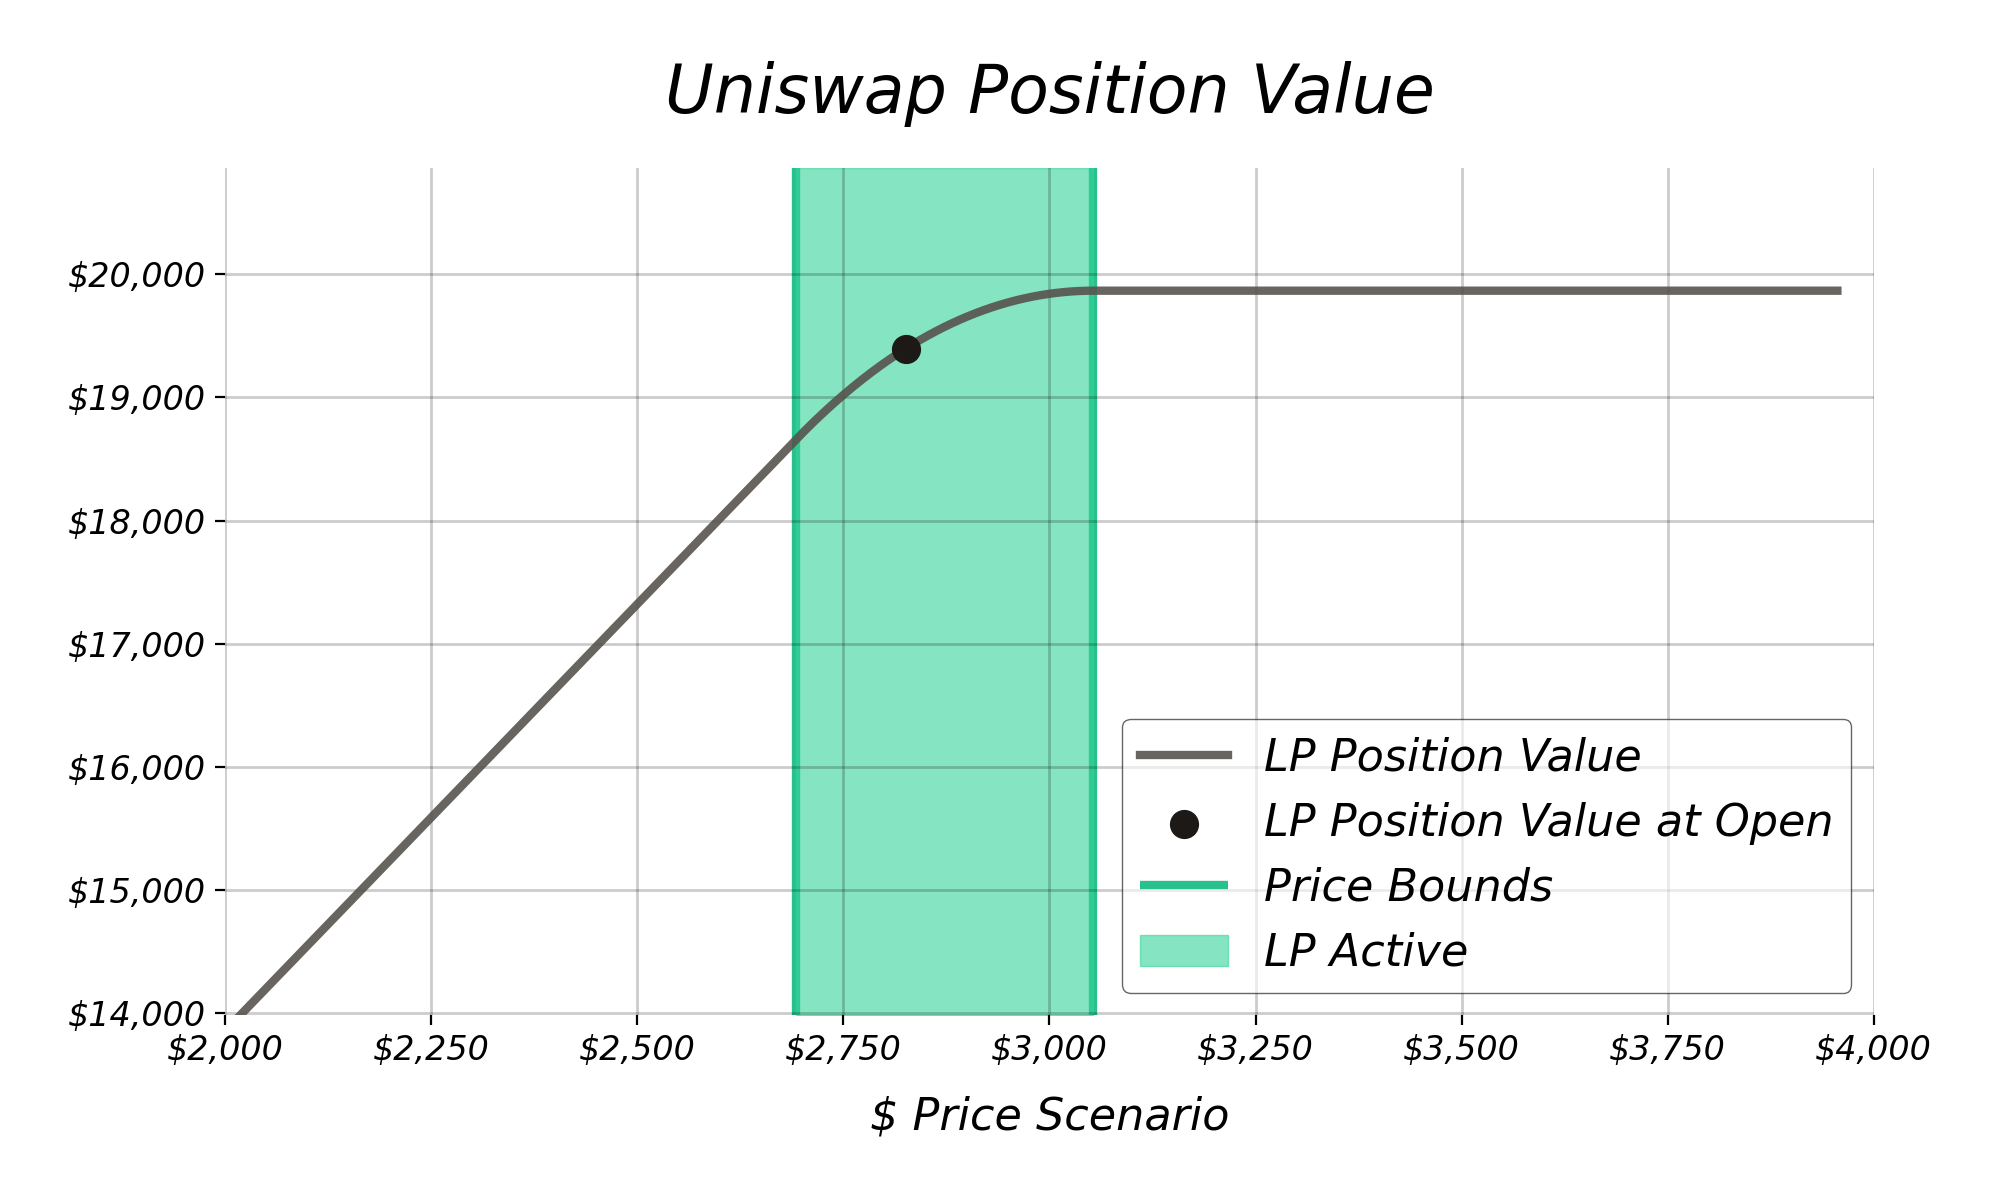
\includegraphics[width=\columnwidth]{img/UniswapPosition.png}
\captionof{figure}{Uniswap LP position value under various ETH price scenarios ($P$).}
\label{fig:lpvalue}
\medskip

As shown in Figure~\ref{fig:lpvalue}, when the ETH price $P$ decreases, the LP position’s value degrades, resulting in impermanent loss. This highlights the need for a hedging strategy to create a market-neutral position, allowing LPs to focus on profitability through collected fees rather than price exposure. 

\subsection{GMX Perpetual Futures}
\label{sec:perphedge}

Perpetual futures are derivative contracts that track the spot price of an asset (here, ETH) without an expiration date, using a funding rate mechanism to balance long and short positions. 

\subsubsection{Perpetual Components}
The following parameters define a GMX perpetual futures contract in this hedging strategy:
\begin{itemize}
	\item \textbf{Entry Price ($P_0$)}: The ETH price (in USDT) at the time the position is opened, serving as the reference for profit and loss (PnL) calculations.
	\item \textbf{Mark Price ($P$)}: The current ETH price, typically derived from an oracle to prevent manipulation, used to calculate unrealized PnL.
	\item \textbf{Collateral ($M$)}: The margin (in USDT) posted to open and maintain the position, determining leverage and liquidation risk.
	\item \textbf{Leverage ($L$)}: The ratio of the position’s notional value to the margin, defined as $L = \frac{\alpha P_0}{M}$. Higher leverage amplifies gains and losses, increasing liquidation risk.
	\item \textbf{Notional Size ($\alpha$)}: The size of the perpetual position (in ETH units), calculated as $\alpha = \frac{L \cdot M}{P_0}$, representing the hedged ETH exposure.
	\item \textbf{Liquidation Price ($P_{\mathrm{liq}}$)}: The ETH price at which liquidation is triggered loss of the entire margin $M$ is occurred. 
	\item \textbf{Funding Rate}: A periodic payment (every hour on GMX) between long and short holders to align the perpetual price with the spot price. Positive rates mean shorts pay longs, while negative rates mean longs pay shorts, impacting profitability.
\end{itemize}

\subsubsection{Perpetual Risks}
Holding Perpetual introduces risks:
\begin{itemize}
    \item \textbf{Delta Risk}: Changes in $P$ can decrease (or increase) the perpetual position’s market value.
	\item \textbf{Liquidation Risk}: If $P$ exceeds $P_{\mathrm{liq}}$, the position is liquidated, resulting in the loss of $M$.
	\item \textbf{Funding Costs}: Persistent positive funding rates can erode profits over time.
\end{itemize}

\subsubsection{Short Perpetual Strategy}
In a short perpetual position, the return increases as the price drops, proportional to the notional size $\alpha$. Liquidation occurs when $P$ rises significantly above $P_0$.\footnote{In practice, GMX may use partial liquidations or maintenance margins, but we assume full liquidation at $P_{\mathrm{liq}}$ for simplicity.}

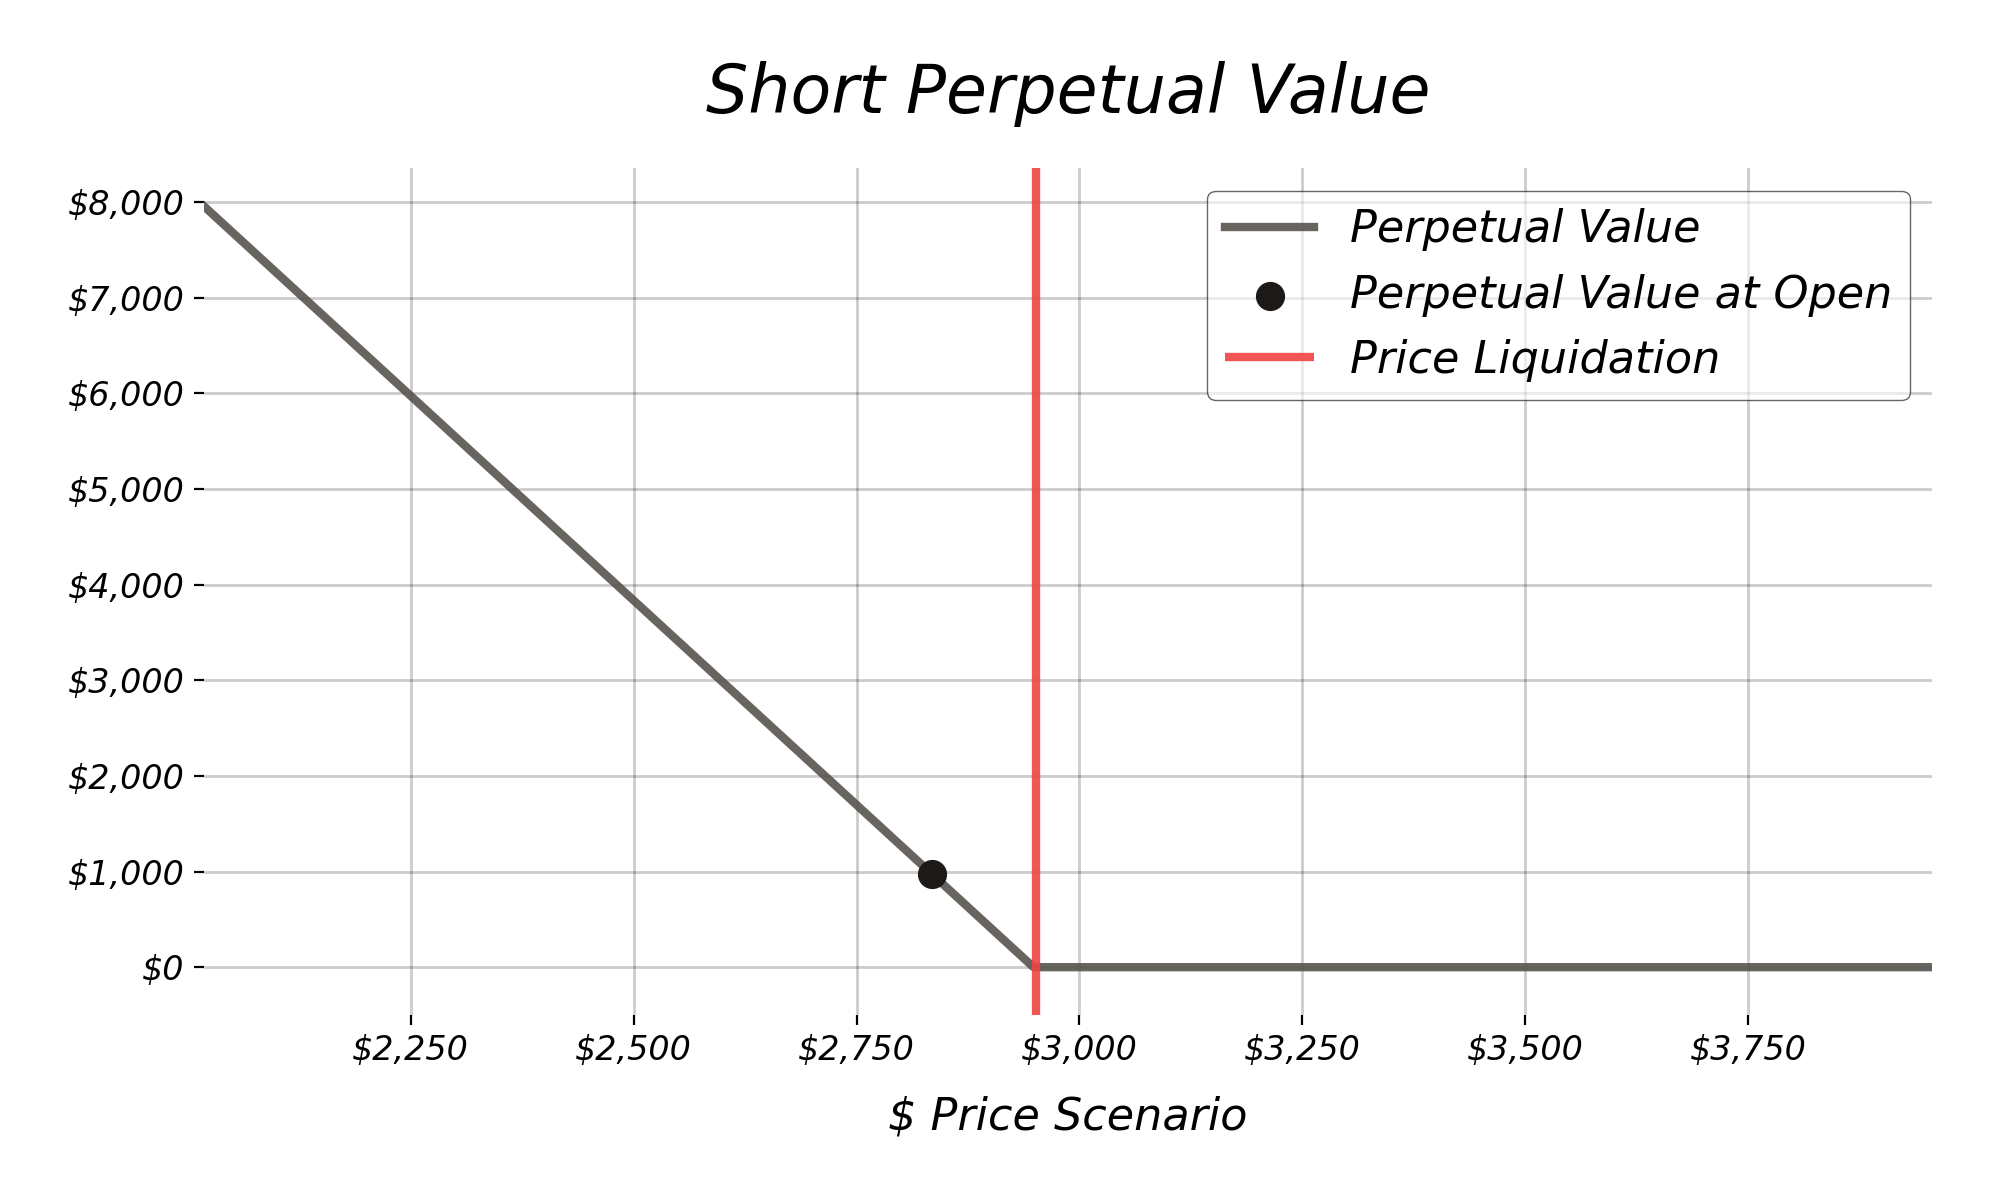
\includegraphics[width=\columnwidth]{img/GMXPosition.png}
\captionof{figure}{Payoff of a short GMX perpetual position under various price scenarios ($P$).}
\label{fig:gmxpayoff}
\medskip
A short perpetual position can offset impermanent loss (IL) when the ETH price drops, as the perpetual’s gains counterbalance the LP’s losses. To mitigate IL in the LP position, we will employ a short perpetual futures contract on the GMX platform. For instance, if $P$ decreases, the LP position incurs IL due to pool rebalancing, but the short perpetual gains $\alpha (P_0 - P)$, compensating for the loss. This approach leverages positive delta risk in perpetual to neutralize the delta risk of the LP position.


\subsection{Integrated LP and Perpetual}
\label{sec:fiveway}

This section evaluates the combined Uniswap V4 LP and short GMX perpetual strategy, aiming to dynamically hedge ETH price exposure while optimizing capital efficiency. The goal is to mitigate impermanent loss (IL) while balancing downside protection and potential gains.

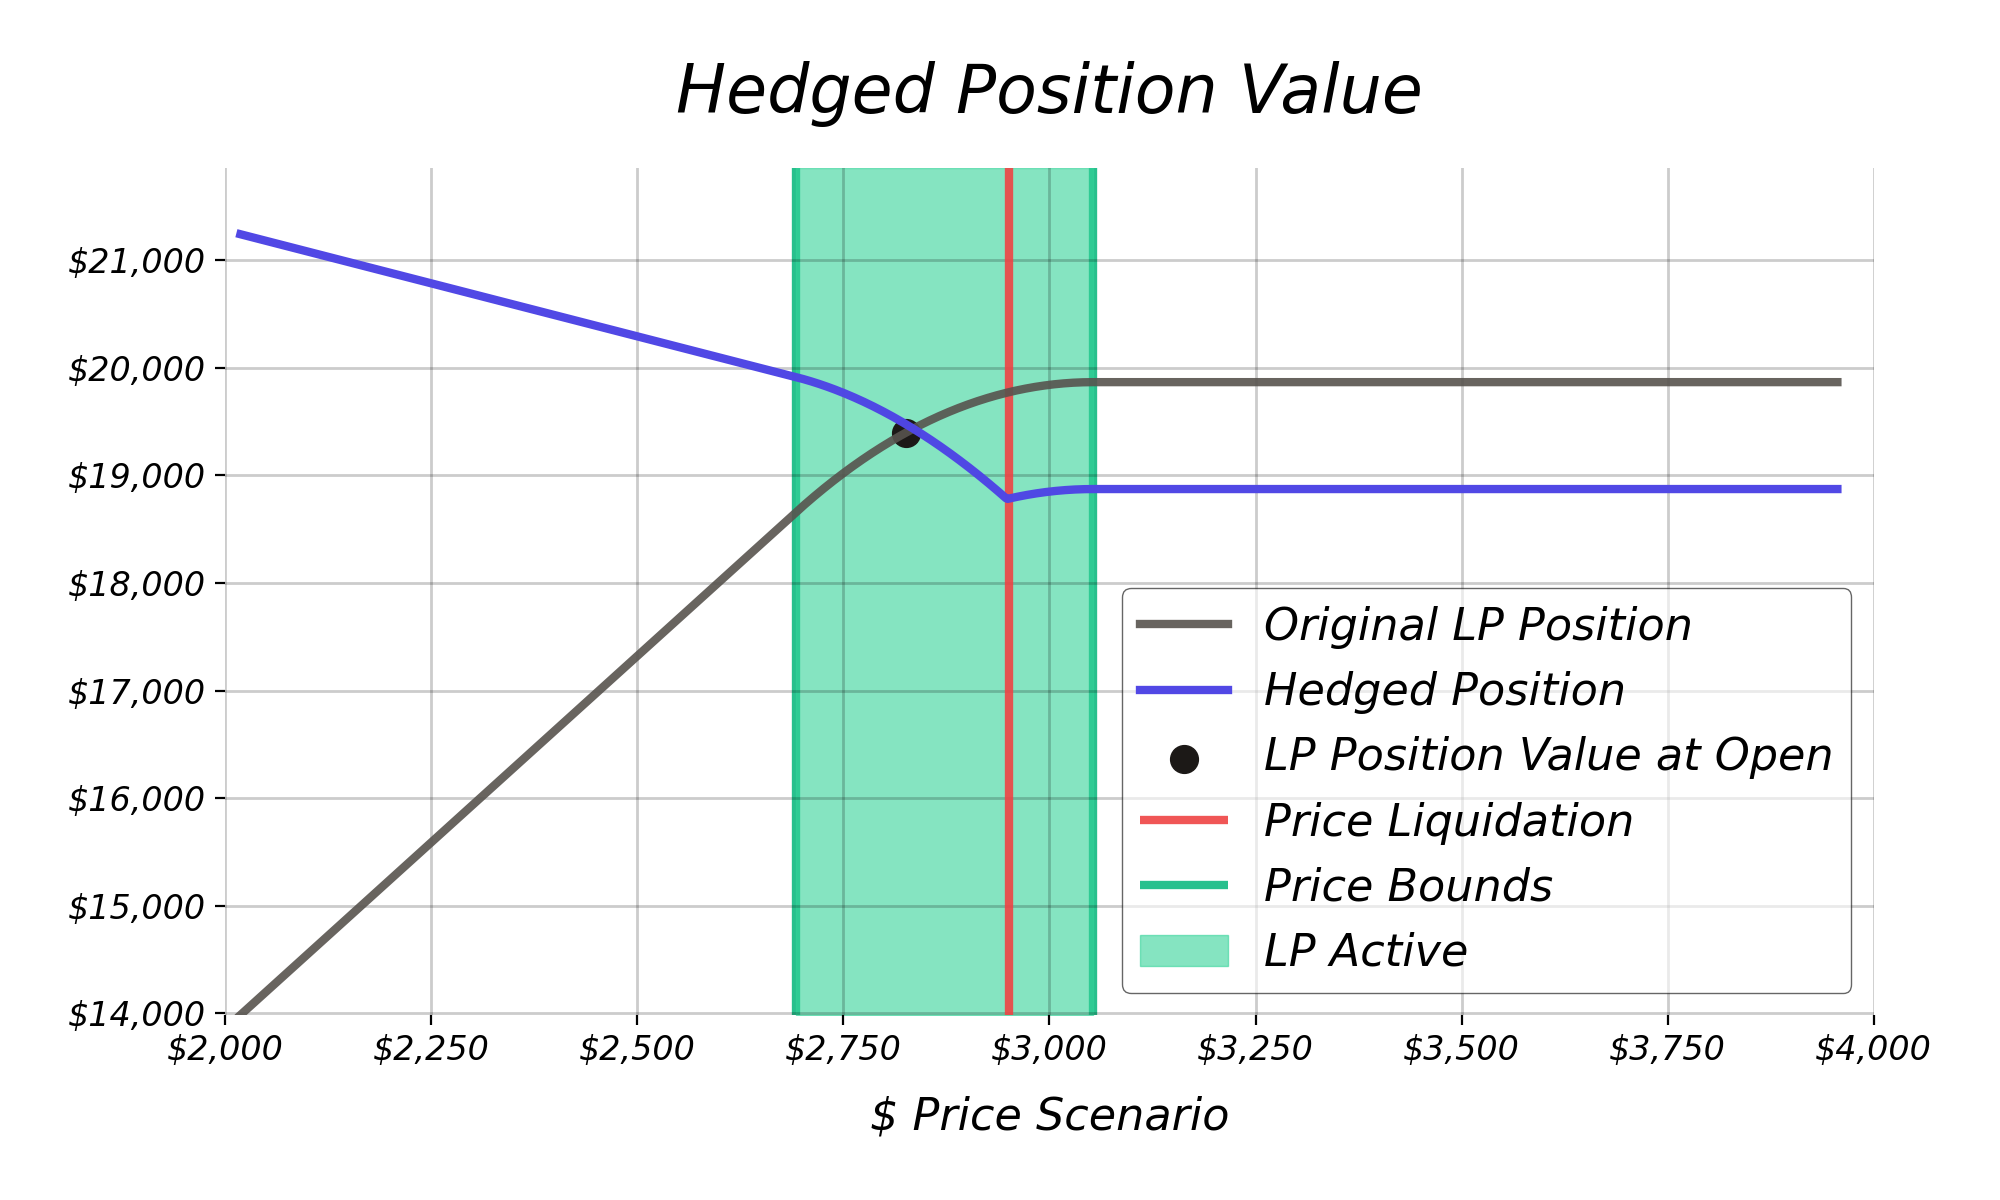
\includegraphics[width=\columnwidth]{img/HedgedPosition.png}
\captionof{figure}{Value of the hedged LP-perpetual position under various ETH price scenarios ($P$).}
\label{fig:perpvalue}
\medskip

As shown in Figure~\ref{fig:perpvalue}, the combined strategy reduces the LP position’s sensitivity to price changes, offering robust protection against IL. Consequently, at a realized price, the LP position’s value remains nearly identical to its value at the entry point, with profits derived primarily from collected fees accumulated during the LP position’s duration.


\subsubsection{Hedging Risks}
However, the strategy’s success depends on careful risk management, considering the following factors:
\begin{itemize}
	\item \textbf{Funding Cost}: The cost of holding a perpetual position increases over time. Therefore, a maximum duration must be established to limit these costs.
	\item \textbf{Collateral Cost}: The cost of entering a position, which is withdrawn from the original LP position. This value must be calibrated to avoid consuming too much of the payoff when the price increases, while remaining sufficient to enable effective hedging when the price decreases.
	\item \textbf{Leverage Adjustment}: Higher leverage amplifies returns but increases sensitivity to price swings, funding costs, and liquidation risk. To ensure efficient hedging, leverage must be adjusted to avoid early liquidations triggered by regular market noise, instead responding to sustained and realized price trends.
\end{itemize}
In summary, the notional size $\alpha$ must balance liquidation risk and capital efficiency. Over-hedging increases exposure to liquidation, while under-hedging fails to mitigate IL. Additionally, an extended holding period may erode profits due to accumulating hedging costs.

\medskip
The maximum holding time and fixed collateral costs will be determined through back-testing. However, leverage adjustments can be dynamically defined using Xtreamly’s volatility predictions.

\subsection{Xtreamly Volatility Forecasting}
\label{sec:xtreamly}

Xtreamly’s volatility forecasting enhances the hedging strategy by informing leverage and risk management decisions, reducing the likelihood of premature liquidation.

\subsubsection{Forecasts of Market States}

Xtreamly categorizes market conditions into three states based on predicted volatility:
\begin{itemize}
	\item \textbf{Low Volatility}: Minimal price movements are expected, allowing for higher leverage.
	\item \textbf{Medium Volatility}: Moderate price movements are anticipated, requiring balanced leverage.
	\item \textbf{High Volatility}: Significant price movements are expected, necessitating lower leverage to avoid liquidation.
\end{itemize}

\subsubsection{Leverage Adjustment}

Although Xtreamly cannot predict exact price movements, it uses volatility forecasts to dynamically adjust leverage when opening perpetual positions. During low-volatility periods, higher leverage can enhance profitability by amplifying the hedge’s effectiveness. In high-volatility periods, lower leverage reduces liquidation risk, ensuring the hedge remains active to protect against IL. This approach will be further explored in the back-testing section.

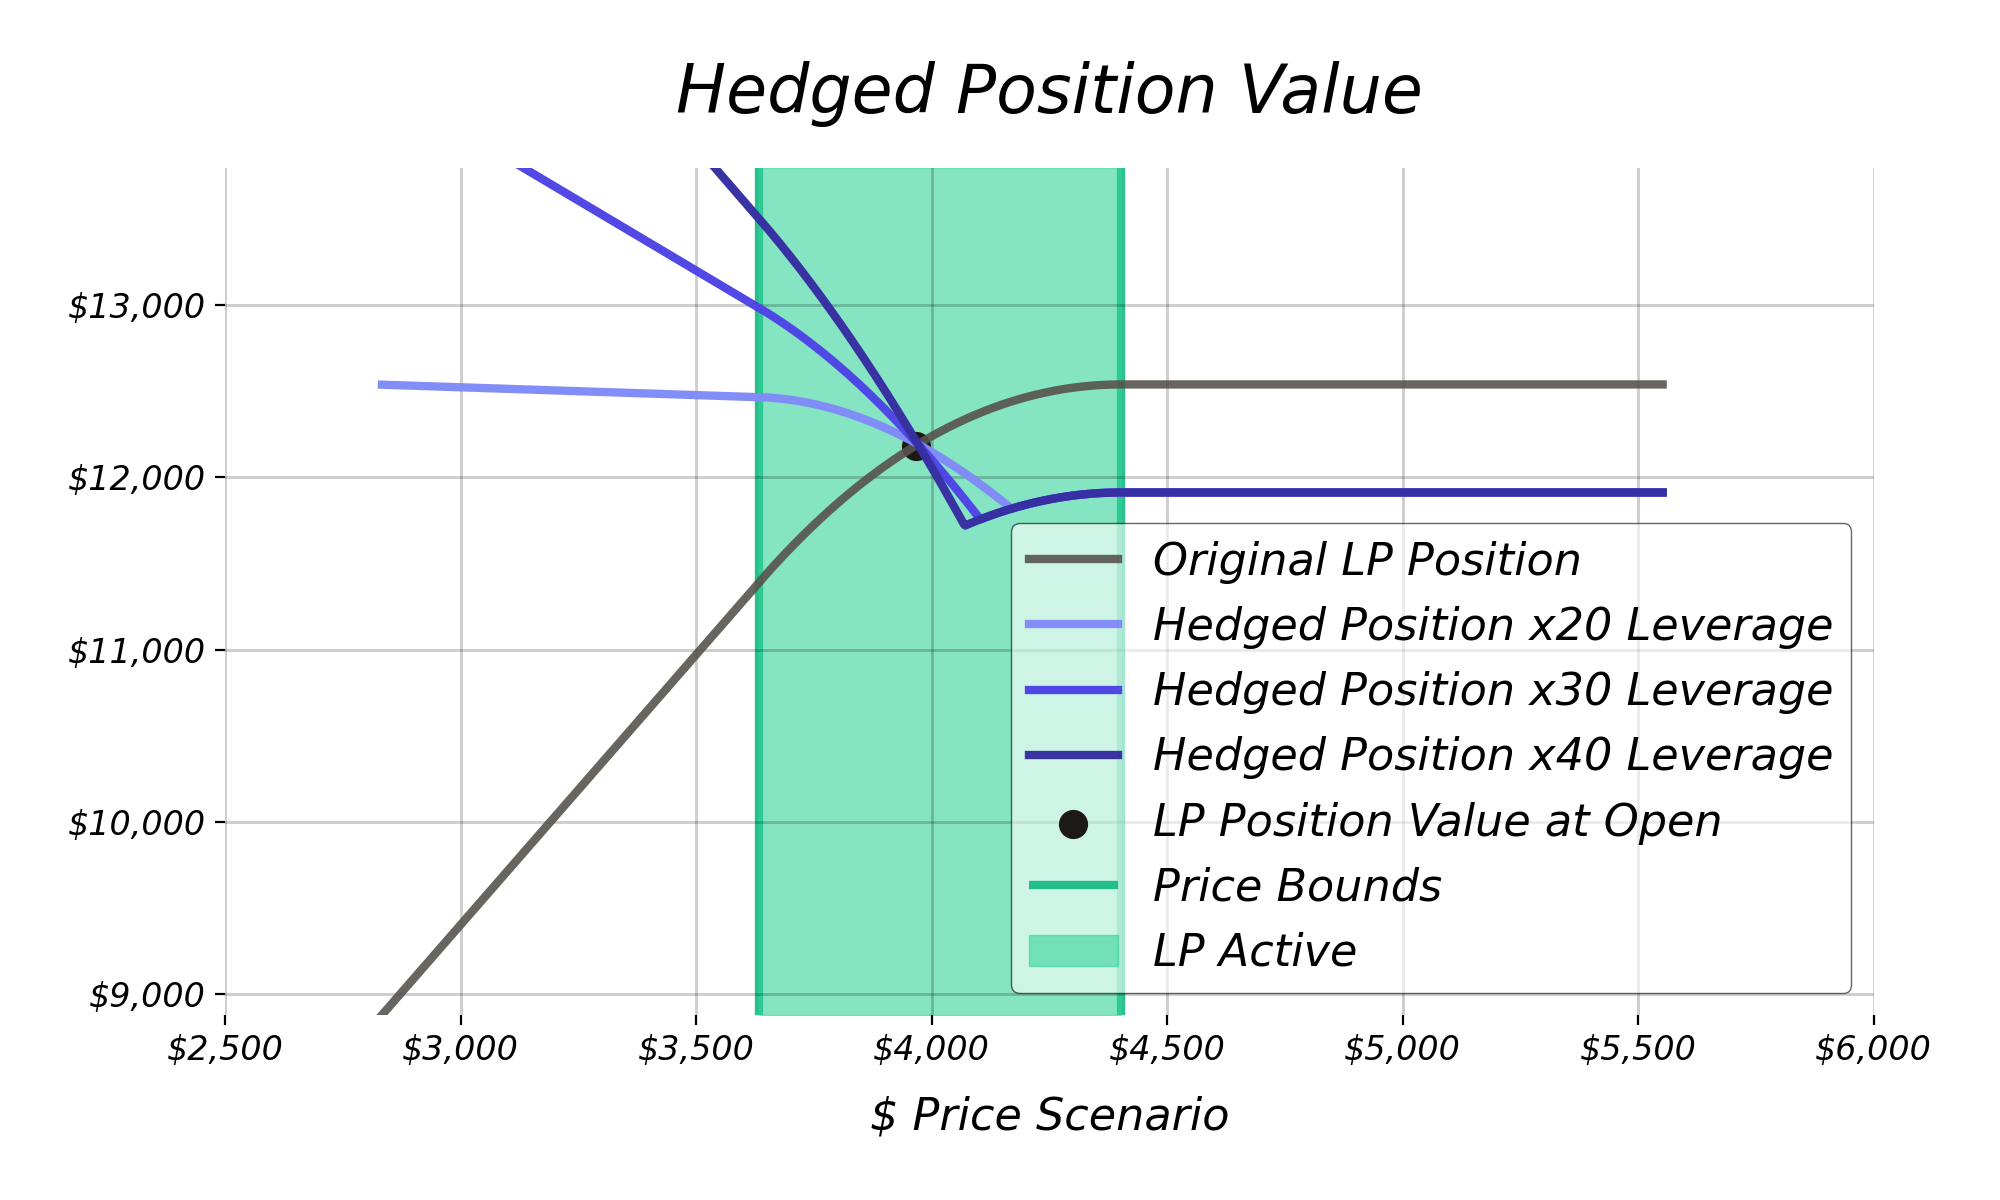
\includegraphics[width=\columnwidth]{img/HedgedPositionLeverage.png}
\captionof{figure}{Payoff of a hedged position with different leverage levels.}
\label{fig:hedgedpayoffleverage}
\medskip

\subsubsection{Increase Returns}
Higher leverage increases positive returns when the price declines. Once liquidations are avoided, the payoff function can also be maximized. Thus, the Xtreamly component is not only critical for determining appropriate leverage but also for maximizing returns whenever the price drops.

\medskip
An alternative scenario would involve minimizing collateral costs based on leverage levels. This approach would maintain a delta-neutral strategy but could result in missed hedging opportunities, therefore, it is skipped.

\newpage

\section{Back-testing}

Back-testing across diverse market scenarios—such as high volatility, trending, or stable conditions—validates the strategy’s robustness and prevents excessive churn.

Back-testing across diverse market scenarios—such as high volatility, trending, or stable conditions—validates the strategy’s robustness and prevents excessive churn.


\subsubsection{Entering Hedge}

The primary motivation for hedging is to mitigate IL. This implies that hedging is most effective when initiated at the start of an LP position and can also be applied whenever the price returns to the entry price level $P_0$. This approach ties the hedging decision directly to price movements and the current perpetual exposure (when no short perpetual position is active).

\medskip

Specifically, the condition for initiating a hedge is defined by the price $P$:
$$\text{Signal}_\text{Hedge} = \frac{P_0}{1.01} <= P \wedge P <= P_0 \cdot 1.01$$ 

This indicates that hedging should be triggered whenever $P$ falls within a 1\% band around $P_0$ and no perpetual position is currently open.

\subsubsection{Optimizing the Hedging Strategy}
Rigorous testing of the LP-perpetual interaction across various market conditions confirms the strategy’s effectiveness and highlights potential weaknesses. The following aspects must be addressed to optimize hedging:

\begin{itemize}
	\item \textbf{Maximum Holding Time}: GMX funding payments, made hourly, can erode profits, particularly if rates consistently favor long positions.
	\item \textbf{Collateral Allocation}: The margin $M$ determines the hedge’s effectiveness. Under-allocating diminishes its impact, while over-allocating is a fundamental cost to original LP position and affect the PnL.
	\item \textbf{Leverage Selection}: For instance, $5\times$ leverage reduces the required $M$ but heightens liquidation risk during price fluctuations.
\end{itemize}

By fine-tuning these parameters, liquidity providers can dynamically adjust their hedging strategy, balancing capital efficiency and risk management across diverse ETH price scenarios.

\newpage

\section{Further Work}
\label{sec:futurework}

\subsection{Further Analysis}
Future research should extend the analysis to a broader range of pools and timelines. This will further validate the strategy’s robustness across various scenarios, including bull and bear markets, and periods of different volatility.

\subsection{AI-Driven Volatility Enhancements}
Integrating Xtreamly’s AI predictive methodology to the intelligence behind opening and closing perpetual positions, in particular:
\begin{itemize}
	\item \textbf{Maximum Drawdown Prediction}: Extend forecasts to maximum drawdown alongside variance to enhance leverage decisions that minimize liquidation risk. 
	\item \textbf{Semivariance and Price Prediction}: Predict volatility in a specific direction (e.g., downside semivariance) to optimize collateral allocation and tailor hedges to directional risks, improving capital efficiency.
	\item \textbf{Funding Rate Prediction}: Model future funding rates to extend the maximum holding time of perpetual positions, reducing the impact of funding costs on hedging profitability.
	\item \textbf{Dynamic Fee Prediction}: Predict Uniswap’s dynamic fees to optimize collateral cost for hedging, by balancing the trade-off between future collected fees and IL. This means, whenever higher collected fees are predicted, the IL is less material. 
\end{itemize}

\subsection{AI-Driven Hedging Signals}
Leverage Xtreamly’s AI predictions to identify additional timing for additional hedging actions. In particular, the system could detect periods with a high likelihood of significant price drops, signaling the need for increased short perpetual exposure.

\subsection{Investment Agent}
Develop an automated investment agent with predefined rules for managing hedging exposure and rebalancing LP positions. This agent will:
\begin{itemize}
	\item \textbf{Rebalance LP positions} by reallocating liquidity across price ranges to keep LP position active.
	\item \textbf{Hedge LP positions} by monitoring real-time market data, adjusting perpetual leverage and notional size to maximize returnss.
\end{itemize}
Such automation would reduce manual intervention, increase scalability, and ensure consistent strategy execution.

\subsection{Hedging with Options}
Integration of DeFi options trading via platforms like Panoptic to complement perpetual-based hedging. Options could secure protection during high-volatility periods, in particular: using put options to hedge against downside IL when prices drop below 

\medskip

This approach would diversify hedging tools, potentially reducing reliance on leverage and funding costs while enhancing protection in extreme market conditions.

\newpage

\section{Appendix}

\bigskip

\subsection{Hedging Mathematics}
\medskip
\subsubsection{LP Position}
Let's consider LP variables:

\begin{itemize}
	\item $P$: The current market price
	\item $P_L$: The lower bound price
	\item $P_U$: The upper bound price
	\item $L$: The \emph{constant} liquidity of the LP position
	\item $X_0$: The amount of $token_0$ held at LP opening
	\item $Y_0$: The amount of $token_1$ held at LP opening
\end{itemize}

\textbf{Ignoring fees}: We assume the LP payoff depends only on the realized price $P$.

\subsubsection{Three Cases for the LP Value}

\paragraph{Case 1: Within Range} $P_L \le P \le P_U$
 
\smallskip

When the market price $P$ lies within the chosen range $[P_L, P_U]$, the position consists of a mix of $token_0$ and $token_1$. The exact amounts of each asset are determined by Uniswap's liquidity formula of $P$:

\begin{align*}
X(P) = L \biggl(\frac{1}{\sqrt{P}} - \frac{1}{\sqrt{P_U}}\biggr)
\end{align*}
\begin{align*}
Y(P) = L \bigl(\sqrt{P} - \sqrt{P_L}\bigr)
\end{align*}

where:
\begin{itemize}
	\item $L$ is the total liquidity provided to the range.
	\item $X(P)$ represents the amount of $token_0$.
	\item $Y(P)$ represents the amount of $token_1$.
\end{itemize}

The LP total value is the value of both tokens:
\[
V_{\text{Case 1}}(P) = X(P) \cdot P \;+\; Y(P).
\]

Expanding:
\begin{align*}
V_{\text{Case 1}}(P) &= L \biggl(\frac{1}{\sqrt{P}} - \frac{1}{\sqrt{P_U}}\biggr) P \\
&\quad + L \bigl(\sqrt{P} - \sqrt{P_L}\bigr),
\quad \text{for } P_L \le P \le P_U.
\end{align*}

\paragraph{Case 2: Below Range} $P < P_L$.
 
\smallskip

When the price drops below $P_L$, the liquidity position has been fully converted into $token_0$. This happens because as price decreases, the Uniswap mechanism sells all available $token_1$ in exchange for $token_0$. So, the $token_0$ amount is locked at the value of $P_L$:
\[
X(P_L) = L \biggl(\frac{1}{\sqrt{P_L}} - \frac{1}{\sqrt{P_U}}\biggr).
\]
The LP holds only $token_0$:
\[
V_{\text{Case 2}}(P) = X(P_L) \cdot P.
\]
Expanding:
\[
V_{\text{Case 2}}(P) = L \biggl(\frac{1}{\sqrt{P_L}} - \frac{1}{\sqrt{P_U}}\biggr) P,
\quad \text{for } P < P_L.
\]

\paragraph{Case 3: Above Range} $P > P_U$.
 
\smallskip

When the price moves above $P_U$, the liquidity position has been fully converted into $token_1$. This happens because as price increases, the Uniswap mechanism sells all available $token_0$ in exchange for $token_1$.

\medskip

The $token_1$ amount is locked at the value it had at $P_U$, which is:
\[
Y(P_U) = L \bigl(\sqrt{P_U} - \sqrt{P_L}\bigr).
\]
The LP holds only $token_1$:
\[
V_{\text{Case 3}}(P) = Y(P_U).
\]
Expanding:
\[
V_{\text{Case 3}}(P) = L \bigl(\sqrt{P_U} - \sqrt{P_L}\bigr),
\quad \text{for } P > P_U.
\]

\paragraph{Final Piecewise Formula.}
 
\smallskip

The complete value function for the LP position is:
\[
V(P) =
\begin{cases}
V_{\text{Case 1}}(P), & \text{for } P < P_L,\\[8pt]
V_{\text{Case 2}}(P), & \text{for } P_L \le P \le P_U,\\[10pt]
V_{\text{Case 3}}(P), & \text{for } P > P_U.
\end{cases}
\]

\smallskip
\centering

\includegraphics[width=0.9\columnwidth]{images/CLposition.png}
\caption{Piece-wise value of a LP position.}
\label{fig:CLposition}
\justifying

\subsubsection{Perpetual Positions}
\label{sec:mathperpetuals}
Let's consider perpetual variables:
\begin{itemize}
	\item $M$: The collateral (in $token_1$) at opening.
	\item $\alpha$: The \emph{notional} size of the perpetual.
	\item $P_0$: The entry price ($token_1$ per $token_0$).
	\item $P_{\mathrm{liq}}$: The liquidation price at which the perpetual is closed and collateral is lost.
\end{itemize}

\paragraph{Short Perpetual}  
 
\smallskip

Suppose we \emph{short} at price $P_0$. The PnL from the short is $\alpha\,(P_0 - P)$. We post margin $M$ to cover losses if $P$ rises. We define $P_{\mathrm{liq}}$ so that when $P = P_{\mathrm{liq}}$, our margin is fully exhausted:
\[
M + \alpha\,(P_0 - P_{\mathrm{liq}}) = 0
\quad\Longrightarrow\quad
P_{\mathrm{liq}} = P_0 + \frac{M}{\alpha}.
\]
Hence, our \textbf{short} payoff is
\[
V_{\mathrm{short}}(P) = 
\begin{cases}
M + \alpha\,(P_0 - P), & P < P_{\mathrm{liq}},\\
-M, & P \ge P_{\mathrm{liq}}.
\end{cases}
\]

\smallskip
\centering

\includegraphics[width=0.9\columnwidth]{images/short.png}
\captionof{figure}{Piecewise payoff for the Short Perpetual, showing the drop to $-M$ at liquidation.}
\label{fig:short}
\justifying
\medskip

\paragraph{Long Perpetual}  
 
\smallskip

If we \emph{long} at $P_0$, the PnL is $\alpha\,(P - P_0)$. The margin $M$ is depleted if $P$ falls by enough. Setting $P = P_{\mathrm{liq}}$ where margin is exhausted:
\[
M + \alpha\,(P_{\mathrm{liq}} - P_0) = 0
\quad\Longrightarrow\quad
P_{\mathrm{liq}} = P_0 - \frac{M}{\alpha}.
\]
Hence, our \textbf{long} payoff is
\[
V_{\mathrm{long}}(P) = 
\begin{cases}
-M, & P \le P_{\mathrm{liq}},\\
\alpha\,(P - P_0), & P > P_{\mathrm{liq}}.
\end{cases}
\]

At liquidation ($P = P_{\mathrm{liq}}$), the payoff \emph{jumps} from some positive level (on the linear portion) down to $-M$, reflecting full loss of the margin. This discontinuous drop represents the complete loss of collateral at the liquidation boundary.

\smallskip
\centering

\includegraphics[width=0.9\columnwidth]{images/long.png}
\caption{Piece-wise payoff for the Long Perpetual, showing the drop to $-M$ at liquidation.}
\label{fig:long}
\justifying
\medskip

\newpage


\subsection{Alternative Strategies}
\label{sec:alternative}

This section explores alternative combinations of an LP position with perpetual hedges and highlights their potential applications.

\medskip
However, these strategies retain the inherent risks of perpetual positions. For instance, if the price oscillates frequently around the entry levels of the perpetual positions, liquidations may occur before meaningful profits are realized. This could lead to accumulated losses, undermining the hedges’ intended purpose of managing long-term exposure.

\subsubsection{Multi Short Perpetual Strategy}

The single short perpetual hedging strategy was discussed in Section~\ref{sec:hedging}.

\centering

\includegraphics[width=0.9\columnwidth]{images/combined_short.png}
\caption{Payoff of an LP position with a short perpetual hedge.}
\label{fig:combined-short}
\justifying

\medskip
In contrast, the Multi Short Perpetual strategy can be applied to pools with two volatile tokens (e.g., BTC and ETH), where the depreciation of one token may result in impermanent loss (IL) denominated in a third currency, such as USDT.

\subsubsection{Long Perpetual Strategy}

\centering

\includegraphics[width=0.9\columnwidth]{images/combined_long.png}
\caption{Payoff of an LP position with a long perpetual hedge.}
\label{fig:combined-long}
\justifying

\medskip
Figure~\ref{fig:combined-long} illustrates the combined payoff of a long perpetual hedge with an LP position. This approach is suitable when exposure to the price appreciation of the underlying asset ($token_0$) is desired. Without a hedge, if the price exceeds the upper bound $P_U$, the LP position fully converts to $token_1$, missing out on further upside potential. By incorporating a long perpetual hedge, the strategy captures additional gains from price increases.

\subsubsection{Combined Perpetual Strategy}

\centering

\includegraphics[width=0.9\columnwidth]{images/combined_both.png}
\caption{Payoff of an LP position with both short and long perpetual hedges.}
\label{fig:combined-both}
\justifying

\medskip
Figure~\ref{fig:combined-both} illustrates the combined payoff of an LP position hedged with both short and long perpetual positions. This configuration aims to protect against both downside and upside price movements, reducing the risk of the LP position moving out of range. While this combined approach provides significant downside protection and potential upside gains, it requires careful risk management to ensure that liquidation losses do not outweigh the hedging benefits.

\end{multicols}

\end{document}